%**************************************************************
% Valutazione MSCRED
%**************************************************************
\label{val-mscred}
Dopo 7 epoche di addestramento, MSCRED ha proposto la soluzione riportata in \hyperref[fig:sol-valid-mscred]{Figura 4.3.} per l'insieme 
di validazione. Evidenziamo come MSCRED riesca a percepire l'andamento improvvisamente anomalo della serie temporale estratta 
dal dataset di Infostud, 
generando anomaly score elevati per ogni punto corrispondente a uno dei ventisei delle anomalie ground-truth, 
evidenziate dall'area rossa. In questo caso, la soluzione ha portato a un risultato perfetto, ottenendo uno score 
F1 pari a 1.0 e affermando l'ipotesi sollevata nel \hyperref[cap2:hypothesis]{Capitolo 2}: il dataset che rappresenta 
le latenze medie è un ottimo indicatore per quanto riguarda l'analisi e l'individuazione delle anomalie.

Riguardo all'insieme di test, MSCRED ha ottenuto risultati leggermente inferiori ma propone comunque una soluzione ottima 
mostrata in \hyperref[fig:sol-test-mscred]{Figura 4.4.} Le metriche risultanti dalla soluzione sono riportate 
nella \hyperref[tab:mscred-metrics]{Tabella 4.4.}

\begin{figure}[H]
    \centering
    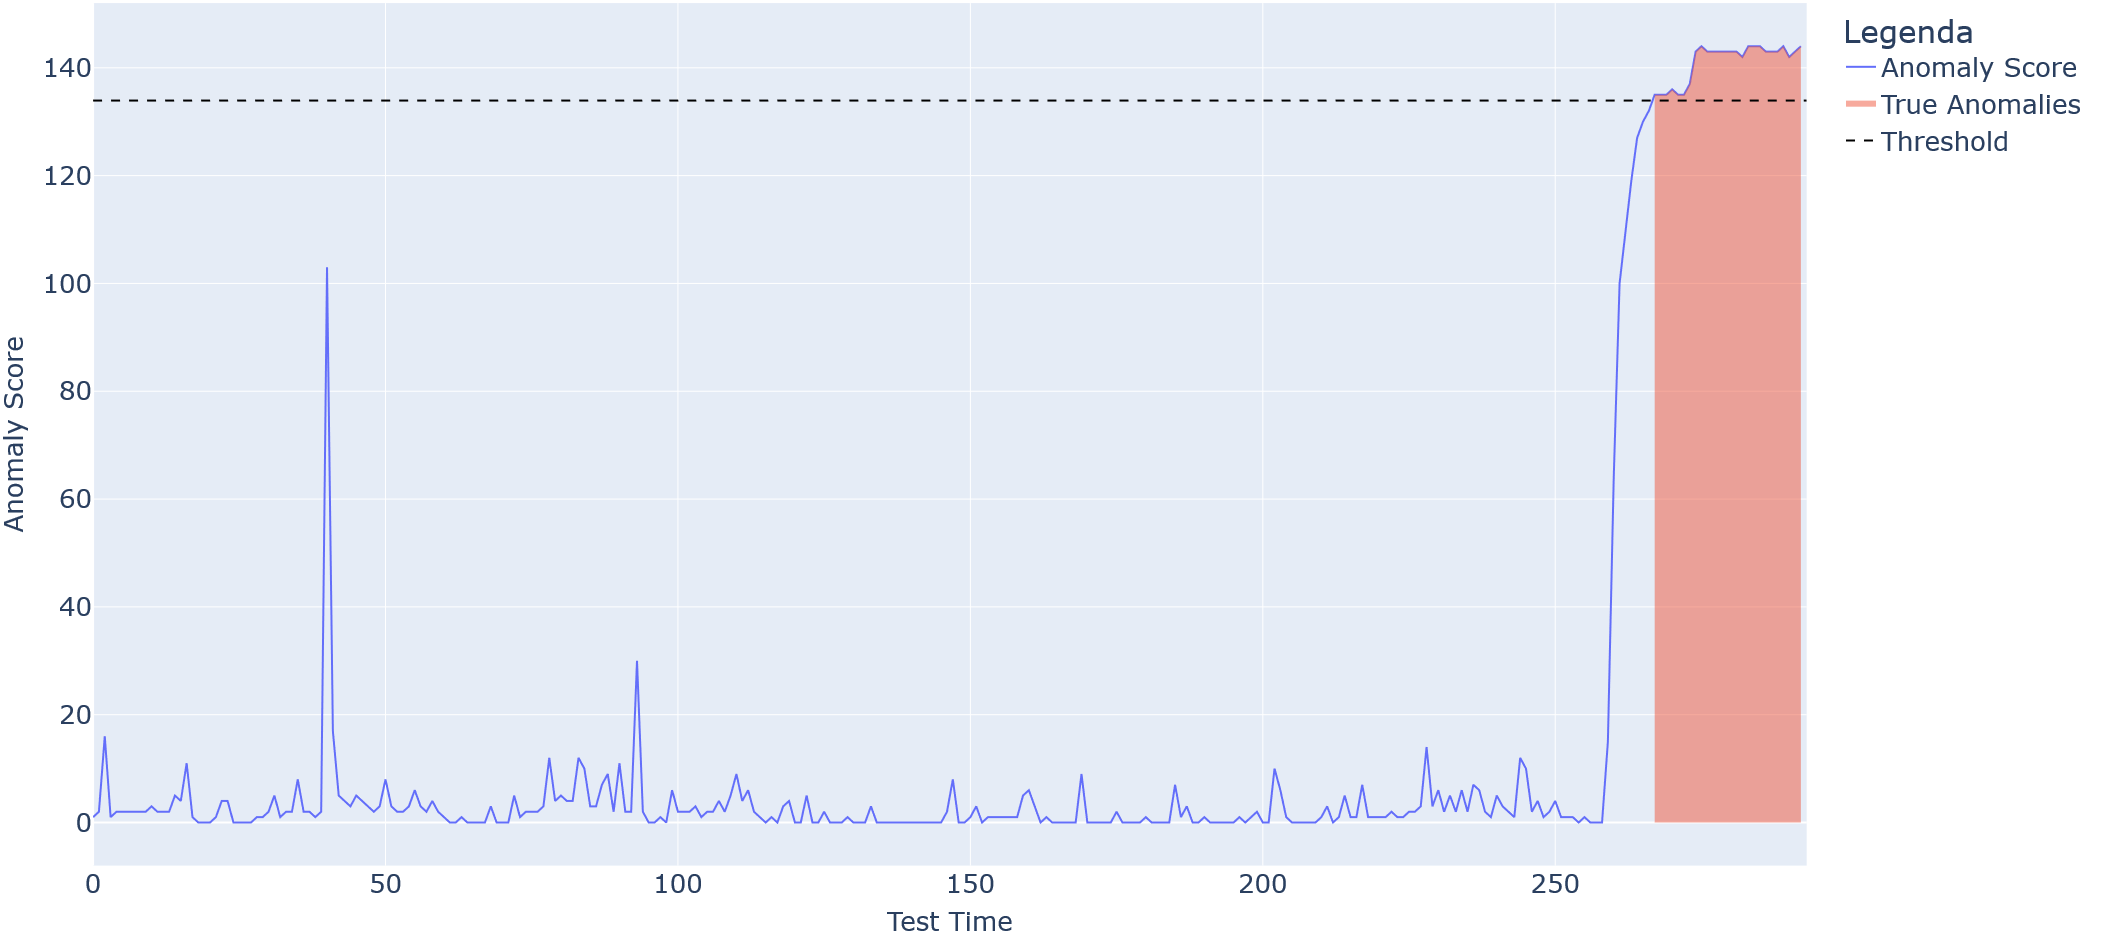
\includegraphics[width=0.7\textwidth]{./input/chapters/models/figs/sol-valid-mscred.png}
    \caption{Soluzione MSCRED sul validation set.}
    \label{fig:sol-valid-mscred}
\end{figure}


\begin{figure}[H]
    \centering
    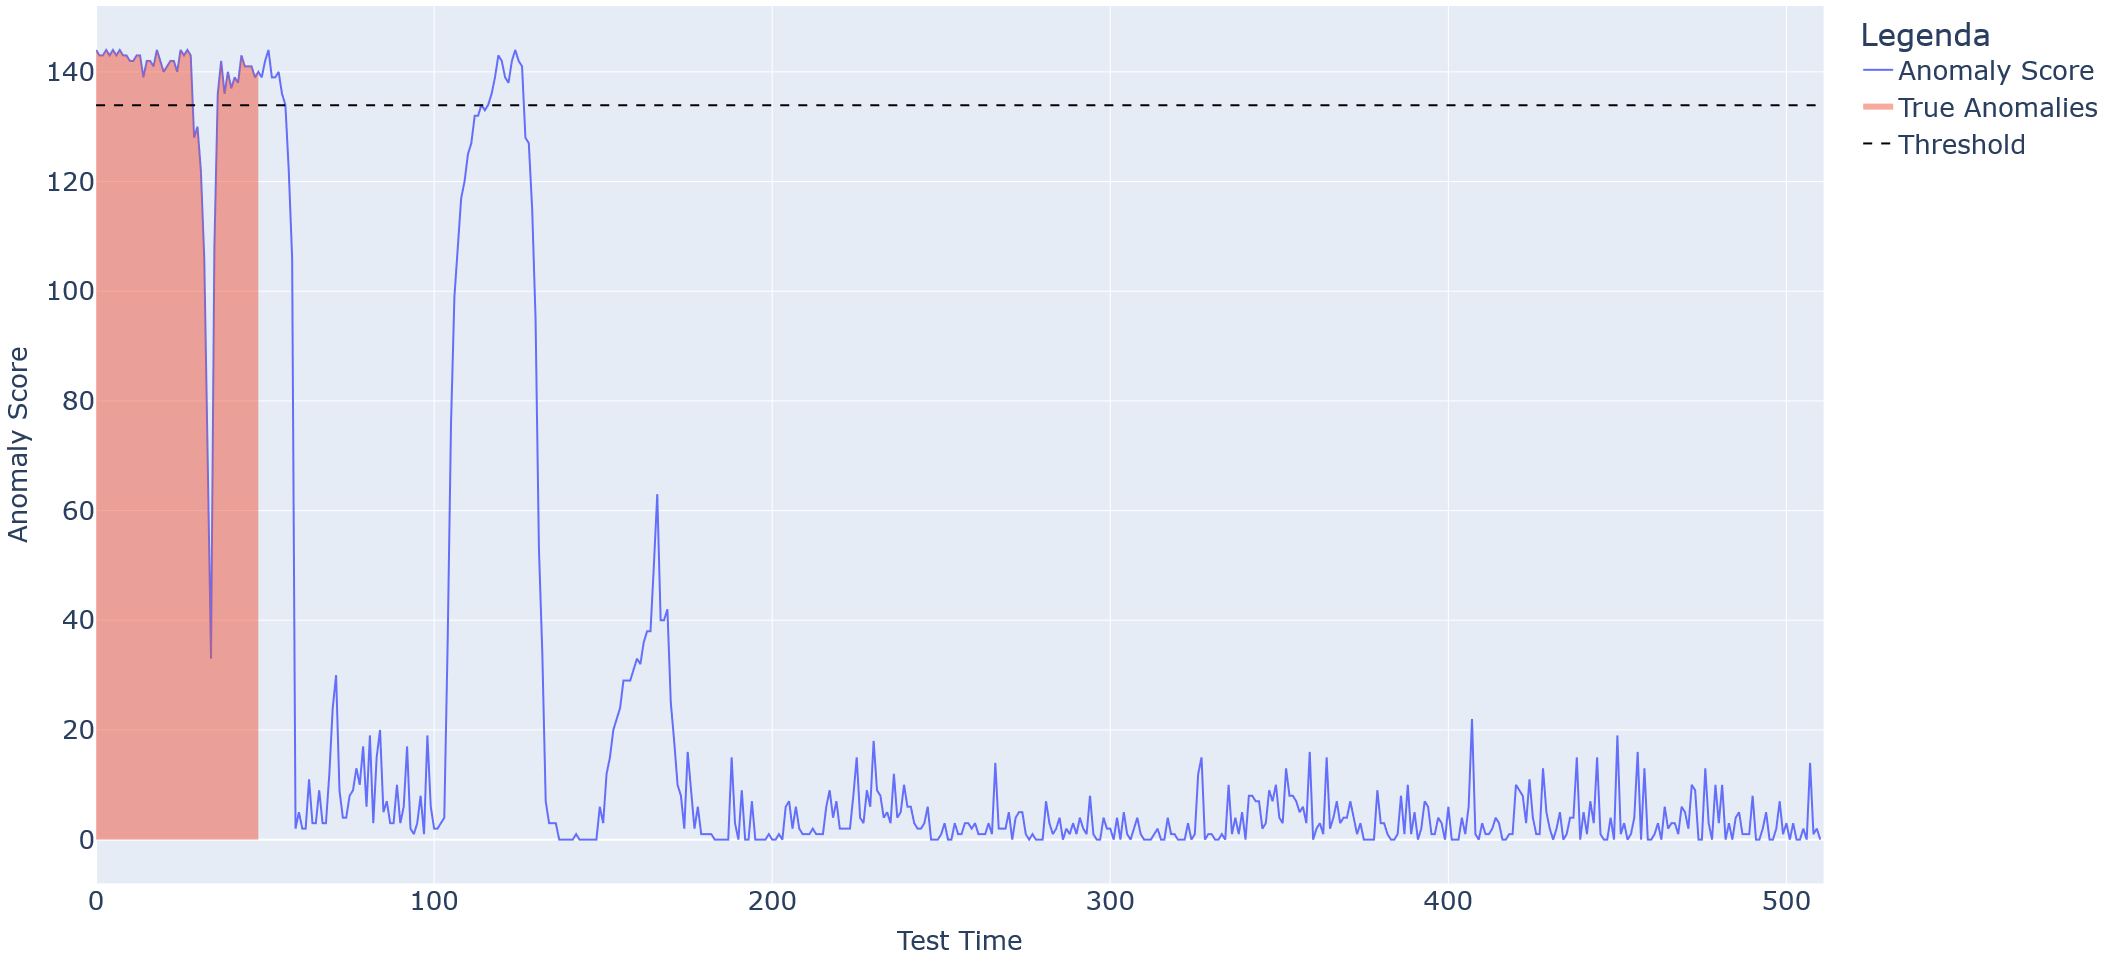
\includegraphics[width=0.7\textwidth]{./input/chapters/models/figs/sol-test-mscred.png}
    \caption{Soluzione MSCRED sul test set.}
    \label{fig:sol-test-mscred}
\end{figure}

\begin{table}[H]
    \centering
    \caption{Risultati MSCRED.}
    \begin{tabular}{lr}
    \toprule
    \textbf{Soluzione MSCRED sul test set}  \\
    \midrule
    \multirow{3}{*}{\textbf{Metriche}} & Precisione: 0.711 \\
    & Recall: 0.857 \\
    & F1-score: 0.777 \\
    \bottomrule
    \end{tabular}
    \label{tab:mscred-metrics}
\end{table}

\paragraph{Conclusioni} I risultati dimostrano in maniera cristallina che MSCRED fornisce
soluzioni notevolmente migliori rispetto agli altri metodi presi in analisi.
Il modello, inoltre, riesce a catturare l'intercorrelazione dei segnali e la dipendenza temporale che
hanno le osservazioni vicine nello spazio, e quindi nel tempo, delle serie temporali multivariate.
MSCRED offre una misura numerica della severità delle anomalie anziché una semplice classificazione binaria, 
soddisfacendo così tutti i requisiti per un algoritmo di rilevamento delle anomalie discussi nel 
\hyperref[cap:intro]{Capitolo 1.} e permettendo all'anomaly detection di compiere un grande passo avanti. 

D'altro canto, però, assumendo che il dataset di Infostud preso in analisi rispetti 
la proprietà IID, MSCRED sembra non offrire soluzioni altrettanto ottimali su serie temporali molto lunghe, ma fa sì che alcune anomalie pesino 
molto più di altre e non garantisce più una netta differenza tra i periodi anomali e non anomali. Questa supposizione 
è basata su delle prove fatte durante il percorso di studio di MSCRED: più è lunga la serie temporale, più 
MSCRED sembra performare in maniera peggiore. Tale affermazione, però, richiede studi più approfonditi per poter 
essere dimostrata o smentita.